\textbf{SON: INTRO THE PROBLEM}

In practice, a configurable system usually provides a large number of
{\bf configuration options} to configure several optional segments of code
to be present or absent, in addition to
\textit{the core} of the system.
%
Those optional segments of code are aimed to realize the
optional \textbf{features} of the system.
%
For example, in Linux Kernel, the configuration options have the
prefix of \texttt{CONFIG\_}, and they can have different
values. Without loss of generality, we assume that the value of a
configuration option is either \texttt{true(T)} or
\texttt{false(F)} (We can consider the entire conditional
  expressions of non-boolean options as boolean ones, e.g.,
  \texttt{CONFIG\_A>10} as \texttt{CONFIG\_A>10=T/F}).

%Code in example_src.c
\begin{figure}
\centering
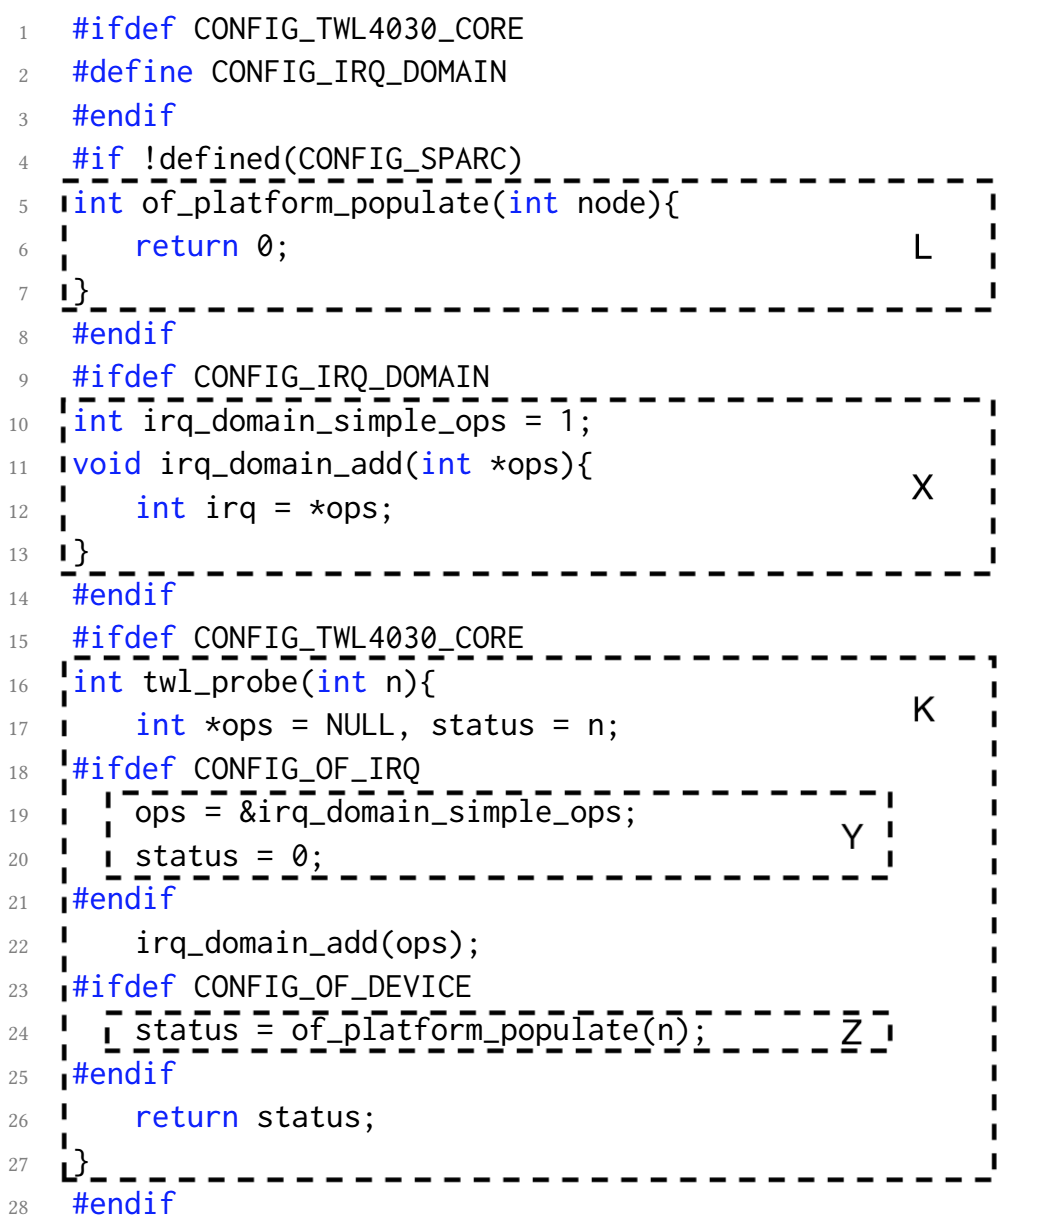
\includegraphics[width=0.5\textwidth]{example_bk.png}
\caption{A simplified buggy version of Linux kernel}
\label{example1}
\end{figure}


\begin{Definition}{({\bf Configuration Option}).}
A configuration option ({\em option} for short) is an element that is used
to configure the source code of a configurable system, such that the
option's value determines the presence or absence of one or more
segments of~code.
\end{Definition}

In a configurable system, the presence or absence of code segments is
dependent on the values of multiple options. In Figure~\ref{example1},
the lines 19 and 20 are presented only when both
\texttt{CONFIG\_TWL4030\_CORE} and \texttt{CONFIG\_OF\_IRQ} are
\texttt{T}. Thus, at line 19, \texttt{irq\_domain\_simple\_ops} is
potentially used to assign as a value to the variable \texttt{ops}
when both above options are \texttt{T}.

%\texttt{CONFIG\_OF\_IRQ} is \texttt{true}.

\begin{Definition}{({\bf Selection Functions}).}
In a configurable system, we define selection functions as the
functions from $O\times V$ to $2^P$, where $O$ is the set of
configuration options, $V=\{\texttt{T, F}\}$, and $P$ is the set of program
entities used in the code of the configurable system. We define four selection functions:

\begin{itemize}

\item $\alpha: O \times V \to 2^P$, $\alpha(o, v) = D$, where $o \in O, v \in \{\texttt{T, F}\}$, and $D$ is the set of entities potentially {\bf declared} if $o = v$.

\item $\beta: O \times V \to 2^P$, $\beta(o, v) = D$, where $o \in O, v \in \{\texttt{T, F}\}$, and $D$ is the set of entities potentially {\bf assigned} if $o = v$.

\item $\gamma: O \times V \to 2^P$, $\gamma(o, v) = D$, where $o \in O, v \in \{\texttt{T, F}\}$, and $D$ is the set of entities potentially {\bf used} if $o = v$.

\item $\delta: O \times V \to 2^P$, $\delta(o, v) = D$, where $o \in O, v \in \{\texttt{T, F}\}$, and $D$ is the set of entities potentially {\bf destructed} if $o = v$.
\end{itemize}

\end{Definition}

For example, in Figure~\ref{example1}:

\begin{itemize}

\item $\alpha($\texttt{CONFIG\_SPARC, F}$)$=$\{$\texttt{GLOBAL.of\_platform\_populate, of\_platform\_populate.node}$\}$

\item $\beta($\texttt{CONFIG\_OF\_IRQ, T}$)$=$\{$\texttt{twl\_probe.ops}$\}$

\item $\gamma($\texttt{CONFIG\_OF\_IRQ, T} $)$=$\{$\texttt{GLOBAL.irq\_domain\_simple\_ops}$\}$

\end{itemize}

\begin{Definition}{({\bf Configuration}).}
Given a configurable system, a configuration is a specific
selection of configuration options, which defines a \textbf{variant}
of the system.
\end{Definition}

Configuration options are used to control the features that are
represented by certain segments of code. For example, in
Figure~\ref{example1}, the feature represented by the segment of code
\texttt{X} (feature \texttt{X}) is enabled if the value of
the configuration option \texttt{CONFIG\_IRQ\_DOMAIN} is \texttt{true},
whereas feature \texttt{Y} is enabled if both \texttt{CONFIG\_OF\_IRQ} and \texttt{CONFIG\_\-TWL4030\_CORE} are \texttt{true}.


The interactions between two features $f_1 \sim OP \times \rho_1$, and
$f_2 \sim OP \times \rho_2$ with $\rho_1 \cap \rho_2 \neq \emptyset$,
can be categorized into nine following kinds of interactions (the
\textit{use-use} case is eliminated):

\begin{itemize}

\item $\exists e \in \rho_1 \cap \rho_2$, $e$ is declared in both $f_1$ and $f_2$ (\textit{declare-declare})

\item $\exists e \in \rho_1 \cap \rho_2$, $e$ is declared in $f_1$ and then assigned in $f_2$ (\textit{declare-assign})

\item $\exists e \in \rho_1 \cap \rho_2$, $e$ is declared in $f_1$ and used in $f_2$ (\textit{declare-use})

\item $\exists e \in \rho_1 \cap \rho_2$, $e$ is declared in $f_1$, and destructed in $f_2$ (\textit{declare-destruct})

\item $\exists e \in \rho_1 \cap \rho_2$, $e$ is assigned in both $f_1$ and $f_2$ (\textit{assign-assign})

\item $\exists e \in \rho_1 \cap \rho_2$, $e$ is assigned in $f_1$ and used in $f_2$ (\textit{assign-use})

\item $\exists e \in \rho_1 \cap \rho_2$, $e$ is assign in $f_1$ and destructed in $f_2$ (\textit{assign-destruct})

\item $\exists e \in \rho_1 \cap \rho_2$, $e$ is used in $f_1$ and destructed in $f_2$ (\textit{use-destruct})

\item $\exists e \in \rho_1 \cap \rho_2$, the entity is destructed in both $f_1$ and $f_2$ (\textit{destruct-destruct})


\end{itemize}


\noindent {\bf Feature Interaction Detection.} In a configurable
system, features (except \textit{the features} in the core of the
system) are controlled by certain configuration options. Thus, if
there exists an interaction among features, the interaction will
be:

\begin{itemize}[leftmargin=4mm]

\item \textit{declare-declare}, there exist two options $o_1, o_2$ and their values $v_1, v_2$, such that $\alpha(o_1, v_1) \cap \alpha(o_2, v_2) \neq \emptyset$

\item \textit{declare-assign}, there exist two options $o_1, o_2$ and their values $v_1, v_2$, such that $\alpha(o_1, v_1) \cap \beta(o_2, v_2) \neq \emptyset$

\item \textit{declare-use}, there exist two options $o_1, o_2$ and their values $v_1, v_2$, such that $\alpha(o_1, v_1) \cap \gamma(o_2, v_2) \neq \emptyset$,

\item \textit{declare-destruct}, there exist two options $o_1, o_2$ and their values $v_1, v_2$, such that $\alpha(o_1, v_1) \cap \delta(o_2, v_2) \neq \emptyset$

\item \textit{assign-assign}, there exist two options $o_1, o_2$ and their values $v_1, v_2$, such that $\beta(o_1, v_1) \cap \beta(o_2, v_2) \neq \emptyset$

\item \textit{assign-use}, there exist two options $o_1, o_2$ and their values $v_1, v_2$, such that $\beta(o_1, v_1) \cap \gamma(o_2, v_2) \neq \emptyset$

\item \textit{assign-destruct}, there exist two options $o_1, o_2$ and their values $v_1, v_2$, such that $\beta(o_1, v_1) \cap \delta(o_2, v_2) \neq \emptyset$

\item \textit{use-destruct}, there exist two options $o_1, o_2$ and their values $v_1, v_2$, such that $\gamma(o_1, v_1) \cap \delta(o_2, v_2) \neq \emptyset$

\item \textit{destruct-destruct}, there exist two options $o_1, o_2$ and their values $v_1, v_2$, such that $\delta(o_1, v_1) \cap \delta(o_2, v_2) \neq \emptyset$

\end{itemize}

\begin{table*}[!h]
\centering
\caption{Different kinds of feature-interaction defects}
\label{bugtypes}
\begin{tabular}{|l|l|l|l|l|}
\hline
&Kind of interaction & Condition & Suspicious selection & Potential violation \\ \hline

1&\textit{declare-declare}&$\alpha(o_1, v_1) \cap \alpha(o_2, v_2) \neq \emptyset$ &$o_1=v_1, o_2=v_2$&Declaration duplication\\ \hline
%2&\textit{declare-assign}&$\alpha(o_1, v_1) \cap \beta(o_2, v_2) \neq \emptyset$&$o_1=v'_1, o_2=v_2$&Assignment without declaration\\ \hline
2&\textit{declare-use}&$\alpha(o_1, v_1) \cap \gamma(o_2, v_2) \neq \emptyset$&$o_1=v'_1, o_2=v_2$&Use without declaration\\ \hline
3&\textit{declare-use}&$\alpha(o_1, v_1) \cap \gamma(o_2, v_2) \neq \emptyset$&$o_1=v_1, o_2=v'_2$&Unused variables/functions\\ \hline
4&\textit{declare-destruct}&$\alpha(o_1, v_1) \cap \delta(o_2, v_2) \neq \emptyset$ &$o_1=v'_1, o_2=v_2$&Destruction without declaration\\ \hline
5&\textit{declare-assign}&$\beta(o_1, v_1) \cap \beta(o_2, v_2) \neq \emptyset$&$o_1=v_1, o_2=v_2$&Assignment without declaration\\ \hline
6&\textit{assign-use}&$\beta(o_1, v_1) \cap \gamma(o_2, v_2) \neq \emptyset$&$o_1=v'_1, o_2=v_2$&Use without assignment\\ \hline
7&\textit{assign-destruct}&$\beta(o_1, v_1) \cap \delta(o_2, v_2) \neq \emptyset$&$o_1=v'_1, o_2=v_2$&Destruction without definition\\ \hline
8&\textit{assign-destruct}&$\beta(o_1, v_1) \cap \delta(o_2, v_2) \neq \emptyset$&$o_1=v_1, o_2=v'_2$&Memory leak\\ \hline
9&\textit{destruct-destruct}&$\delta(o_1, v_1) \cap \delta(o_2, v_2) \neq \emptyset$&$o_1=v_1, o_2=v_2$&Destruction duplication\\ \hline
10&\textit{destruct-use}&$\delta(o_1, v_1) \cap \gamma(o_2, v_2) \neq \emptyset$&$o_1=v_1, o_2=v_2$& Use after destruction\\ \hline
\end{tabular}
\end{table*}



\subsubsection{Configuration Prioritization Algorithm}

In general, to prioritize a given set of configurations under test,
our algorithm assigns a suspicious score to a configuration. The
score is determined via the number of the potential
feature-interaction bugs in different kinds that a variant
corresponding to that configuration might have.

\begin{algorithm}
\caption{Feature-Interaction aware Configuration Prioritization Algorithm}	
 \label{agl1}
\begin{algorithmic}[1]
\Procedure {DetectSuspiciousSelections}{$Code$}
\State $Options = ExtractOptions(Code)$
\ForAll {$o \in Options$}
\State $TSelc = CollectProgramEntities(o, T, Code)$
\State $FSelc = CollectProgramEntities(o, F, Code)$
\State $Selections.add(TSelc)$
\State $Selections.add(FSelc)$
\EndFor

\ForAll {$selc \in Selections$}
	\ForAll {$other \in Selections$}
			\If {$ExistInteraction(selc, other)$}
				\If {$IsSensitiveInteraction(selc, other)$}
					\State $ss=ExtractSuspiciousSelection(selc, other)$
					\State $SuspiciousSelections.add(ss)$
				\EndIf
			\EndIf
	\EndFor
\EndFor
\EndProcedure
\Statex

\Procedure {Prioritize}{$Configurations$, $SuspSelections$}
\ForAll {$c \in Configurations$}
	\State $SScore = CaculateSuspiciousScore(c, SuspSelections)$
	\State $SetScore(c, SScore)$
\EndFor
\State $OrderBySuspiciousScoreDesc(Configurations)$
\EndProcedure
\end{algorithmic}
\end{algorithm}


Feature-interaction bugs can be induced by any kinds of
interaction. Table~\ref{bugtypes} shows 10 different kinds of
feature-interaction bugs that are potentially caused by the respective
kinds of feature interactions listed in
Section~\ref{sec:formulation}. The interactions in
Table~\ref{bugtypes} are called \textit{sensitive interactions} with
their \textit{suspicious selection} of options.
%which could potentially lead to the problems for the configurations
%containing it as listed in Section~3.
A configuration containing a suspicious selection potentially has the
corresponding violation.

The listing~\ref{agl1} shows the pseudo-code of the approach, our
feature-interaction aware configuration prioritization
algorithm. Given a configurable system under test, we first extract
the set of options used in the system. Then, for each selection $v$ of
each option $o$, the sets $\alpha(o, v), \beta(o, v), \gamma(o,v)$,
and $\delta(o,v)$ are computed via the function
$CollectProgramEntities$ (lines 4--5). To identify these sets of
program entities, our algorithm analyzes the code by using
\textit{TypeChef}, a variability-aware
parser~\cite{Kenner:2010:TTT:1868688.1868693}. After that, for each
pair of option selections, it detects the potential interactions among
the features and checks whether the interactions are sensitive as
described in Table~\ref{bugtypes}.
%
Sensitive interactions are used to specify suspicious selections. This
information is used to compute suspicious score for each configuration
selected to be tested (line 16). This score is the number of
suspicious selections contained by a configuration, and equal to the
number of potential bugs that  the corresponding variant might
have. Finally, the configurations are sorted descendingly by
their suspicious~scores.